\documentclass[tikz]{standalone}

\usepackage[latin1]{inputenc}
\usepackage{tikz}
\usetikzlibrary{quotes,angles,calc,decorations.markings,patterns,decorations.pathreplacing,arrows.meta}

\tikzset{% adapted from hobby_doc.tex
   show controls/.style={
    decoration={
     show path construction,
     curveto code={
      \draw [blue, -{Circle[black,open]}] (\tikzinputsegmentfirst) -- (\tikzinputsegmentsupporta) ;
      \draw [blue, {Circle[black,open]}-] (\tikzinputsegmentsupportb) -- (\tikzinputsegmentlast) ;
     }
    },decorate
   },
}
% GNUPL
% Draw line annotation
% Input:
%   #1 Line offset (optional)
%   #2 Line angle
%   #3 Line length
%   #5 Line label
% Example:
%   \lineann[1]{30}{2}{$L_1$}
\newcommand{\lineann}[4][0.5]{%
    \begin{scope}[rotate=#2, blue,inner sep=2pt]
        \draw[densely dashed, blue!40] (0,0) -- +(0,#1)
            node [coordinate, near end] (a) {};
        \draw[densely dashed, blue!40] (#3,0) -- +(0,#1)
            node [coordinate, near end] (b) {};
        \draw[|<->|] (a) -- node[] {\contour{white}{#4}} (b);
    \end{scope}
}

\newcommand{\outann}[4][0.5]{%
    \begin{scope}[rotate=#2, blue,inner sep=2pt]
        \draw[densely dashed, blue!40] (0,0) -- +(0,#1)
            node [coordinate, near end] (a) {};
        \draw[densely dashed, blue!40] (#3,0) -- +(0,#1)
            node [coordinate, near end] (b) {};
        % \draw[|<->|] (a) -- node[] {\contour{white}{#4}} (b);
        \draw[->|] ($(a)-(0.1,0)$) -- (a);
        \draw[->|] ($(b)+(0.1,0)$) node[above] {\contour{white}{#4}} -- (b);
        % --  (b);
    \end{scope}
}

\newcommand{\outinann}[4][0.5]{%
    \begin{scope}[rotate=#2, blue,inner sep=2pt]
        \draw[densely dashed, blue!40] (0,0) -- +(0,#1)
            node [coordinate, near end] (a) {};
        \draw[densely dashed, blue!40] (#3,0) -- +(0,#1)
            node [coordinate, near end] (b) {};
        \draw[draw=none] (a) -- node[] {\contour{white}{#4}} (b);
        \draw[->|] ($(a)-(0.1,0)$) -- (a);
        \draw[->|] ($(b)+(0.1,0)$) -- (b);
        % --  (b);
    \end{scope}
}

\newcommand{\lineannOnly}[4][0.5]{%
    \begin{scope}[rotate=#2, blue,inner sep=2pt]
        \draw[densely dashed, blue!40] (0,0) -- +(0,#1)
            node [coordinate, near end] (a) {};
        \draw[densely dashed, blue!40] (#3,0) -- +(0,#1)
            node [coordinate, near end] (b) {};
        % \draw[|<->|] (a) -- node[] {\contour{white}{#4}} (b);
    \end{scope}
}
\usepackage[outline]{contour}
\contourlength{1.2pt}
\colorlet{myblue}{cyan!40!white}
\begin{document}
\pagestyle{empty}

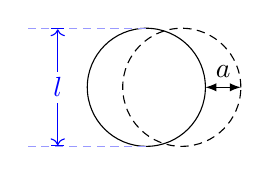
\begin{tikzpicture}[
    scale=1.5, 
    arrowline/.style={black!60},
    kos/.style={black},
    tangent/.style={
        decoration={
            markings,% switch on markings
            mark=
                at position #1
                with
                {
                    \coordinate (tangent point-\pgfkeysvalueof{/pgf/decoration/mark info/sequence number}) at (0pt,0pt);
                    \coordinate (tangent unit vector-\pgfkeysvalueof{/pgf/decoration/mark info/sequence number}) at (1,0pt);
                    \coordinate (tangent orthogonal unit vector-\pgfkeysvalueof{/pgf/decoration/mark info/sequence number}) at (0pt,1);
                }
        },
        postaction=decorate
    },
    use tangent/.style={
        shift=(tangent point-#1),
        x=(tangent unit vector-#1),
        y=(tangent orthogonal unit vector-#1)
    },
    use tangent/.default=1
    ]

\draw[] (0,0) arc [ start angle=0,   
                              end angle=360,
                              x radius=0.5, 
                              y radius=0.5]
        coordinate [pos=0.06,sloped] (1a) {}  
        coordinate [pos=-0.06,sloped] (1b) {} 
        coordinate [pos=.235] (2) {}  
        coordinate [pos=.0] (3) {} 
        coordinate [pos=.76] (4) {};

\draw[xshift=0.3cm, densely dashed] (0,0) arc [ start angle=0,   
                              end angle=360,
                              x radius=0.5, 
                              y radius=0.5]
        coordinate [pos=0.06,sloped] (1a) {}  
        coordinate [pos=-0.06,sloped] (1b) {} 
        coordinate [pos=.235] (2) {}  
        coordinate [pos=.0] (3') {} 
        coordinate [pos=.76] (4) {};

\draw[<->,>=latex] (3) -- node[above] {$a$} (3');

% \draw (3) node[left=0.5em] {$S_1$};

% \draw[rotate around={-10:(2,-1)}, xshift=3cm, scale=0.4, yshift=-2cm] (0,0) arc [ start angle=0,   
%                               end angle=360,
%                               x radius=0.5, 
%                               y radius=1]
%         coordinate [pos=0] (1') {} 
%         coordinate [pos=.25] (2') {} 
%         coordinate [pos=-0.56,sloped] (3'a) {} 
%         coordinate [pos=0.56,sloped] (3'b) {} 
%         coordinate [pos=.75] (4') {} node[right] {$S_2$};

% % \draw (1) to [out=-30, in=180-10] (1');
% \draw (2) to [out=-40, in=180-10] node[sloped,pos=0.5]{\tikz{\draw[->](0,0) -- ++(0.1,0)}} (2');
% \draw (4) to [out=-20, in=180] node[sloped,pos=0.5]{\tikz{\draw[->](0,0) -- ++(0.1,0)}} (4');

% \draw (1a) to [out=-35, in=180-10] node[sloped,pos=0.5]{\tikz{\draw[->](0,0) -- ++(0.1,0)}} (3'a);
% \draw (1b) to [out=-25, in=180-5] node[sloped,pos=0.5]{\tikz{\draw[->](0,0) -- ++(0.1,0)}} (3'b);

% \draw[densely dashed] (3) to [out=-35, in=180-5]  (1');

% \begin{scope}
%     \clip[rotate=-30] (0,0) arc [ start angle=0,   
%                               end angle=360,
%                               x radius=0.5, 
%                               y radius=1];
% \draw[] (3) to [out=-35, in=180-5]  (1');
% \end{scope}
% \begin{scope}
%     \clip[rotate around={-10:(2,-1)}, xshift=3cm, scale=0.4, yshift=-2cm] (0,0) arc [ start angle=0,   
%                               end angle=360,
%                               x radius=0.5, 
%                               y radius=1];
% \draw[] (3) to [out=-35, in=180-5]  (1');
% \end{scope}

% \draw[draw=none,fill=blue!20] (0,0) rectangle (1,1);
% \draw (0,1.2) -- (0,0) -- (1,0) -- (1,0.2) coordinate (A) (1,0.3) coordinate (B) -- (1,1.2);
% \draw (0.5,1) node [above] {$S$};
% \begin{scope}[xshift=1cm, yshift=0.2cm]
%     \outann[0.2]{90}{0.1}{$\sigma$}
% \end{scope}
\begin{scope}[xshift=-0.5cm, yshift=-0.5cm]
    \contourlength{2.1pt}
    \lineann[1]{90}{1}{$l$}
\end{scope}
% \begin{scope}[xshift=1cm, yshift=0cm]
%     \contourlength{2.1pt}
%     \outinann[-0.9]{90}{0.3}{$h_1$}
% \end{scope}
% \fill[myblue] (B) -- (A) to [out=0, in=90] (1.3,0) -- (1.35,0) to [out=90, in=0] (B);
% \draw[blue!40] (A) to [out=0, in=90] (1.3,0);
% \draw[blue!40] (B) to [out=0, in=90] (1.35,0);
% \draw (0,1) -- (0,1);
% \draw[pattern=north east lines, draw=none, pattern color=blue] (0,0) rectangle (2,-0.2);
% \draw[thick, black] (0,0) -- (2,0);

% \draw (0.2,1) -- ++ (-45:0.5) coordinate (A);
% \draw (0.5,1) -- ++ (-45:0.7) coordinate (B);


% \fill[myblue] (2,0.2) .. controls ($(2,0.2)+(0:-0.7)$) and ($(B)+(-45:0.2)$) .. (B) -- (0.5,1) -- (0.2,1) -- (A) .. controls ++(-45:0.4)  and ++(0:0.5) .. (0,0.2) -- (0,0) -- (2,0) -- cycle;

% \draw[blue!40] (0.2,1) -- ++ (-45:0.5) coordinate (A);
% \draw[blue!40] (0.5,1) -- ++ (-45:0.7) coordinate (B);


% \draw[blue!40] (B) .. controls ++(-45:0.2)  and ++(0:-0.7) .. (2,0.2);
% \draw[blue!40] (A) .. controls ++(-45:0.4)  and ++(0:0.5) .. (0,0.2);

% \draw[<-] (0.37,1) ++ (135:0.1) -- ++ (135:0.2) node [above] {$\vec{v}_0$};

% \draw[->] (0.3,1) ++ (-45:0.5) to [out=-45,in=0,looseness=1.4] ++ (-0.2,-0.5);
% \draw[->] (0.4,1) ++ (-45:0.5) to [out=-45,in=180] ++ (0.75,-0.5);
% \draw (0,0) -- ++(3,0);
% \draw (0,0.8) -- ++(1-0.1,0) ++ (0.2,0) -- ++(1-0.2,0) ++ (0.2,0) -- ++ (0.9,0);

% \draw[fill=blue!20,draw=none] (1-0.1,0.4) rectangle ++(0.2,1);
% \draw[black] (1-0.1,0.4) -- ++(0,1.5);
% \draw[black] (1+0.1,0.4) -- ++(0,1.5);

% \draw[fill=blue!20,draw=none] (2-0.1,0.4) rectangle ++(0.2,1.4);
% \draw[black] (2-0.3,0.5) -- (2-0.1,0.5) -- ++(0,1.4);
% \draw[black] (2+0.1,0.4) -- ++(0,1.5) (2+0.1,0.4) -- ++ (0,-0.1) -- ++ (-0.4,0);

% \draw[black, opacity=0.8] (2-0.3,0.4) ellipse (0.04 and 0.1);
% \draw[black, opacity=0.8] (1,0.4) ellipse (0.1 and 0.04);

% \draw[->] (0,0.4) -- ++ (0.4,0);



% \begin{scope}[xshift=2cm, yshift=1.4cm]
%     \lineann[0.65]{90}{0.4}{$\Delta h$}
% \end{scope}
% \begin{scope}[xshift=1cm, yshift=1.4cm]
%     \lineannOnly[-0.76]{90}{0.4}{$\Delta h$}
% \end{scope}


% \draw (1,0) -- ++(0,1);
% \draw (2,0) -- ++(0,1);
% \draw (3,0) -- ++(0,1);

\end{tikzpicture}


\end{document}